% Stand-alone protocol supplement. Select main.tex for the main manuscript.
\documentclass[10pt,twocolumn,letterpaper]{article}
\usepackage[review]{cvpr}
\usepackage{amsmath,amssymb,graphicx,microtype,booktabs}
% Standard figure* floats; the legacy cuted teaser preamble is not needed.
\definecolor{cvprblue}{rgb}{0.21,0.49,0.74}
\usepackage[pagebackref,breaklinks,colorlinks,allcolors=cvprblue]{hyperref}
\hypersetup{pdftitle={FLEX-UF: Supplementary Methods and Controlled Experiments},pdfauthor={Anonymous research draft},pdfsubject={DCVC-UF intra spatial early exit}}
\def\paperID{DRAFT}
\def\confName{CVPR}
\def\confYear{2027}
\renewcommand{\thesection}{S\arabic{section}}
\renewcommand{\thefigure}{S\arabic{figure}}
\renewcommand{\thetable}{S\arabic{table}}
\renewcommand{\theequation}{S\arabic{equation}}
\title{FLEX-UF: Supplementary Methods and Controlled Experiments}
\author{Anonymous research draft}
\begin{document}
\maketitle
\section{Scope and Reproduction}

This supplement records CPU analyses of the frozen evaluation archive and a
prospective protocol for the ongoing depth study. The main manuscript uses
the recorded mixed reconstructions of the shared-latent e15 codec. The new
control-path and spatial-assignment analyses reuse its stored source-error
tables. They produce candidate decisions for later replay, without executing
the codec or measuring new inference times. The independent D2/D4/D6 training
continues separately; no intermediate checkpoint is treated as a completed
depth experiment.

The stand-alone paper repository contains the plotted source tables, source
hash manifests, editable figure scripts and inspection results under
\texttt{data/refresh20260927}. Figures can be regenerated on CPU using
\texttt{scripts/build\_figures.py} and
\texttt{scripts/build\_extended\_figures.py}. The parent research repository
also retains the scripts that derive these summaries from the raw records
and checkpoints. Hashes identify the files inspected during this revision;
they do not retrospectively establish the exact executable used by a
historical run whose code hash was not recorded.

\section{Tracing the Reconstruction Reference}

Two measurement paths need to be distinguished. The source-table producer
loads the e15 network and a separate released-weight reference. It computes
the candidate tile errors $M_{t,k}$ from e15 and the scalar reference error
$R$ from the released synthesis network, both on the padded source.
The final-reconstruction evaluator instead loads e15 alone, calls its
full-frame synthesis path, crops both full and mixed outputs, and measures
their difference in source quality. Its raw field named
\texttt{psnr\_release} is consequently a fine-tuned full-depth reference
in the inspected code (\cref{fig:anchors}).

A CPU comparison of the two state dictionaries finds 255 shared
encoder/entropy tensors with no changes. All 143 inherited synthesis tensors
that can be compared have changed, with a maximum absolute parameter
difference of 0.2481. Thus the reporting path cannot be identified with
released synthesis merely because it executes all twelve trunk blocks.

This distinction limits the interpretation of threshold crossings. The
recorded 7/263 RGB and 49/263 YUV losses above a nominal 0.1\,dB target combine
differences in reference, image support, metric and the influence of the
shared repair/head. They do not identify the contribution of any single
factor. The paired MAC accounting remains attached to the same recorded
maps, but the exact quality gap to the cropped released decoder cannot be
recovered from the exported JSON alone.

The required replay should retain both full-depth anchors, the padded and
valid-pixel errors, and the final mixed reconstruction. Selection and final
verification must use the same declared reference and metric. A failed plan
should trigger an explicit fallback whose bytes and runtime are recorded.

\begin{figure*}[t]
\centering
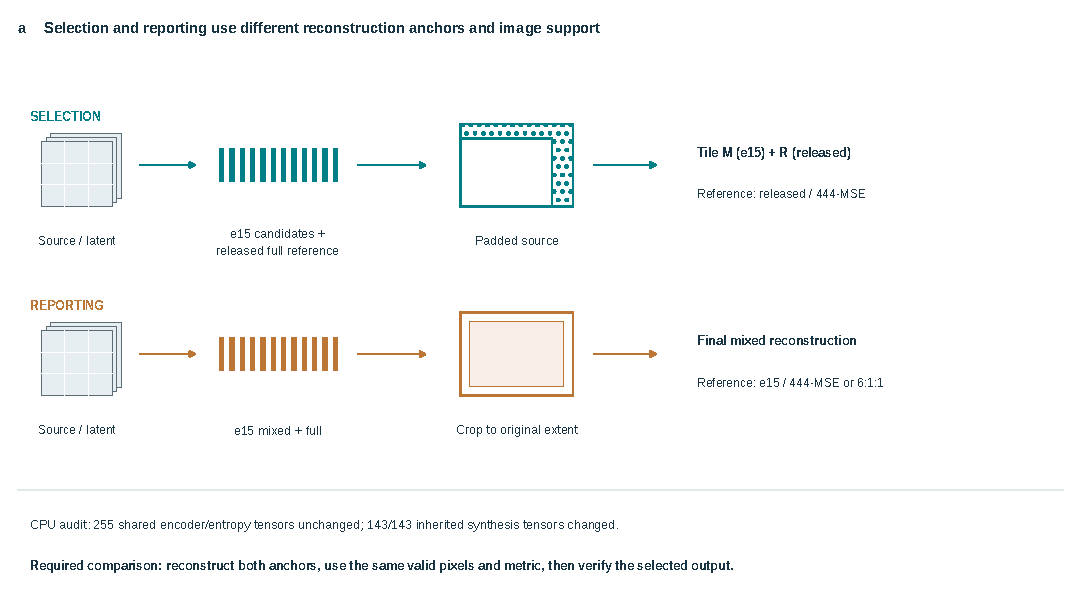
\includegraphics[width=\textwidth]{figs/extended20260927/figS1_reference_protocol.pdf}
\caption{\textbf{Reference and support are part of the measurement.}
Candidate tile errors come from e15, whereas the table denominator comes
from a separate released-weight reference. Final reporting uses the cropped
full-depth e15 reconstruction. The CPU tensor comparison establishes a
weight difference in the inspected checkpoints. The figure traces code
paths and does not depict newly decoded images.}
\label{fig:anchors}
\end{figure*}

\section{Auditing the Scalar Control Search}

For router scores $\ell_{t,k}$ and costs $c_k$, increasing the price $\beta$
in $k_t(\beta)=\arg\max_k(\ell_{t,k}-\beta c_k)$ cannot increase selected cost.
To see this, write the optimality inequalities at $\beta_1<\beta_2$ for
their respective choices $k_1,k_2$ and add them. The result is
\begin{equation}
 (\beta_2-\beta_1)(c_{k_1}-c_{k_2})\geq 0.
\end{equation}
No corresponding statement follows for source error $M_{t,k}$, because that
quantity is absent from the score being optimised. A feasibility test at the
most expensive endpoint can therefore miss a feasible middle assignment,
and distortion-based bisection can miss a later feasible interval.

We enumerate pairwise score-line intersections, representatives of the open
intervals between them, and the endpoints of the archived range
$[-20000,20000]$. Archived controls are included explicitly to retain their
floating-point tie behaviour. Identical maps are merged. Among feasible
maps, the selected candidate maximises modelled MAC saving, with table loss
as a tie-breaker. This is a finite-path audit in float64, rather than an
optimiser over all possible tile assignments.

The cost is monotone on every inspected router path, while source loss has
at least one reversal on 227/265 paths. At 0.05\,dB, enumeration improves
3 of 204 previously feasible plans, by 0.1626 percentage points on average,
and recovers one additional feasible case. At 0.1\,dB it improves 2 of 263
plans, by 0.0277 points on average. No paired saving changes at the four
larger targets. The largest missed saving is 30.45 points at 0.05\,dB, so a
small mean difference should not be read as a uniform per-frame bound.

We strengthen the blind baseline in the same way. For ordered dithering,
all changes occur at a finite set of Bayer-rank thresholds and rung
boundaries. Enumerating those maps reveals source-loss reversals on 232/265
paths. It improves 3/204 paired plans at 0.05\,dB and 1/263 at 0.1\,dB,
with mean gains of 0.0192 and 0.0028 points, respectively. Six additional
cases become feasible at 0.05\,dB. The quality of these newly selected maps
has not been measured after final mixed reconstruction, so they do not
replace the main manuscript's reconstruction curves.

The audit reproduces every archived feasible control and cost, verifies
cost monotonicity, and checks that enumeration never discards a better
archived feasible saving. An independent three-exit example verifies the
non-monotone failure mechanism against a dense control grid.

\section{Separating the Histogram from Spatial Placement}

A map can save arithmetic by selecting many cheap exits even if their
locations contain no useful information. To isolate placement, let
$p_k=N^{-1}\sum_t\mathbf{1}[k_t=k]$ be its fixed exit histogram and let
$\pi$ be a uniformly random permutation of its assignments. Each tile has
marginal exit probability $p_k$, giving the exact expectation
\begin{equation}
 \mathbb{E}_{\pi}\!\left[\frac1N\sum_t M_{t,k_{\pi(t)}}\right]
 =\frac1N\sum_t\sum_k p_k M_{t,k}.
 \label{eq:permutation}
\end{equation}
We report $G=10\log_{10}(\mathbb E_\pi[\overline M_\pi]/\overline M)$,
where $\overline M$ is the recorded map's table MSE. Positive $G$ indicates
useful spatial placement at exactly the same histogram and MAC cost.
The logarithm is outside the expectation: this is not expected PSNR over
random reconstructions.

At 0.1\,dB, source-informed search has a mean placement gain of 0.0321\,dB,
the router 0.0213\,dB, and dithering 0.0007\,dB over their respective shuffled
histograms. The router's 95\% sequence-cluster interval is
[0.0167,0.0262]\,dB; dithering's is [$-0.0002$,0.0017]\,dB. Uniform-depth
maps have zero gain by construction. Among the 263 paired router maps,
204 have positive gain, seven have negative gain and 52 use one exit only.
This diagnoses content association conditional on a source-calibrated
histogram; it does not validate held-out autonomous calibration.

For each map we also solve the exact fixed-histogram assignment problem on
$M$. Repeating each exit column according to its count produces a square
linear assignment problem. Its minimum table MSE gives a conditional upper
bound on placement value. The router's mean regret to that optimum is
0.0044\,dB at the 0.1\,dB target. Every source-search map attains its own
fixed-histogram optimum, as expected for a separable Lagrangian minimiser.
The optimum still requires the complete source table and carries the same
information-acquisition cost. Replaying shuffled and optimal maps through
the mixed decoder is the next required ablation.

\begin{figure*}[t]
\centering
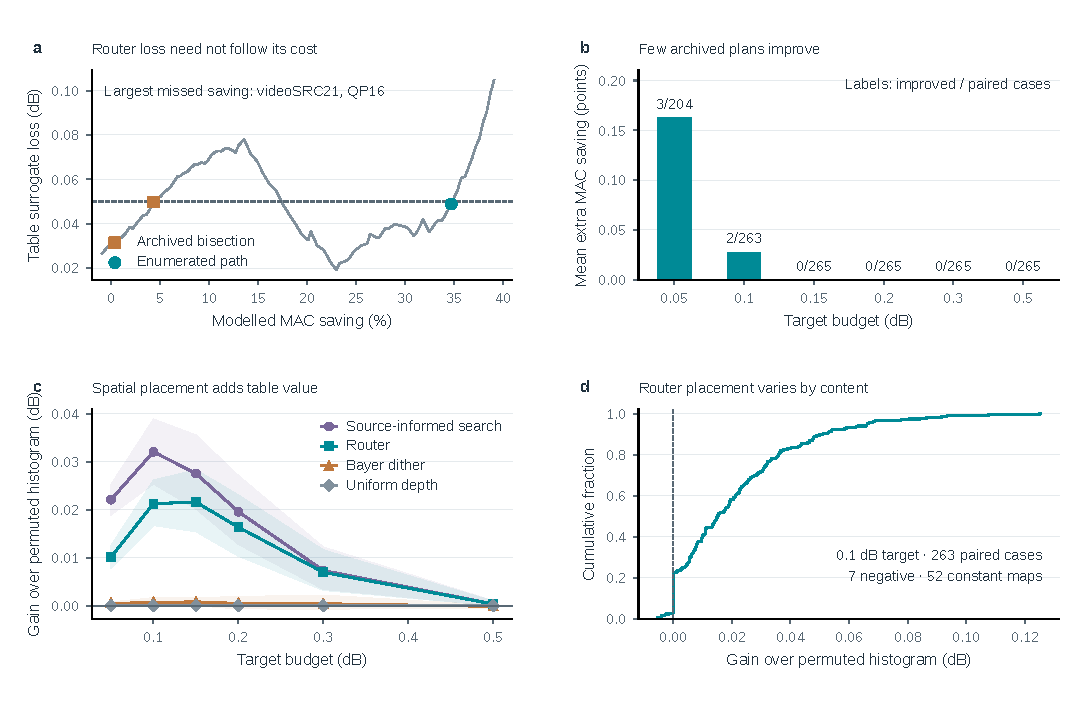
\includegraphics[width=\textwidth]{figs/extended20260927/figS2_control_and_assignment.pdf}
\caption{\textbf{Control-path and assignment diagnostics.}
\textbf{a}, The explicitly selected largest missed router saving illustrates
non-monotone table loss. \textbf{b}, Mean paired improvement from enumerating
the router path; labels show improved and paired counts. Newly feasible
cases are excluded from these means. \textbf{c}, Exact expected-shuffle
comparison at unchanged exit histograms, with 95\% sequence-cluster
intervals. \textbf{d}, Router placement-gain distribution at 0.1\,dB.
All results are CPU analyses of padded error tables; none measures new
final-image quality or latency.}
\label{fig:control}
\end{figure*}

\section{The Independent Depth Study}

The ongoing experiment retains the first two, four or six synthesis trunk
blocks of the DCVC-UF intra architecture and trains each complete codec
under the pinned official recipe. The encoder and entropy weights learn
alongside the decoder. Each model consequently has its own representation,
distinct from the shared-latent exits evaluated in the main paper.
\Cref{fig:bank} shows a possible later deployment path, not an implemented
six-expert result.

\paragraph{Isolating depth.}
Released D12 is a useful deployment anchor, but a D12 trained with the same
data manifest, 105-epoch schedule, optimisation and initialisation protocol
is necessary to isolate depth from training history. D8 and D10 should be
prioritised after the initial depth frontier and this control are available.
The main runs retain the official recipe; distillation and prefix
initialisation are separate variants rather than silent training changes.

\paragraph{Isolating routing.}
The evaluation should progress from full-frame D12 to patchwise D12, the
best validation-selected fixed expert, blind mixtures, simple image
statistics, the MLP and source-informed search. Full-frame versus patchwise
D12 measures the cost of tiling and entropy resets before routing receives
credit for any gain. A histogram-preserving shuffle separates the chosen
expert proportions from their spatial placement.

\paragraph{A concrete router hypothesis.}
A lightweight encoder-side predictor can estimate each expert's distortion
and rate relative to a cheap reference. Given measured runtime tables, a
candidate decision score is
\begin{equation}
 \widehat J_k=\widehat D_k+\lambda\widehat R_k+
 \mu T_k(n_k,\mathrm{shape}).
 \label{eq:proposed}
\end{equation}
Here $n_k$ is the number of patches assigned to expert $k$; grouped execution
can make runtime depend on the assignment as a whole. The score is therefore
a proposed approximation requiring measured validation, rather than an
independent per-patch latency oracle. Regression or regret-weighted training
should be compared against ordinary exit-label cross-entropy. A second-stage
top-two verification can be restricted to small predicted margins, with
its threshold selected on held-out calibration images and its extra encoding
work included in the total.

Spatial competition between complete codecs already provides a close
precedent~\cite{blard2026spatial}; adaptive compression and patch early exit
provide further controls~\cite{tao2023adanic,hu2023cgslim,wang2022ape}.
The testable direction here is depth-heterogeneous selection with measured
rate--distortion--time costs and reduced encoder search. Practical codec
studies motivate including device execution and perceptual
assessment~\cite{jia2025dcvcrt,tatwawadi2026practical}.

\begin{figure*}[t]
\centering
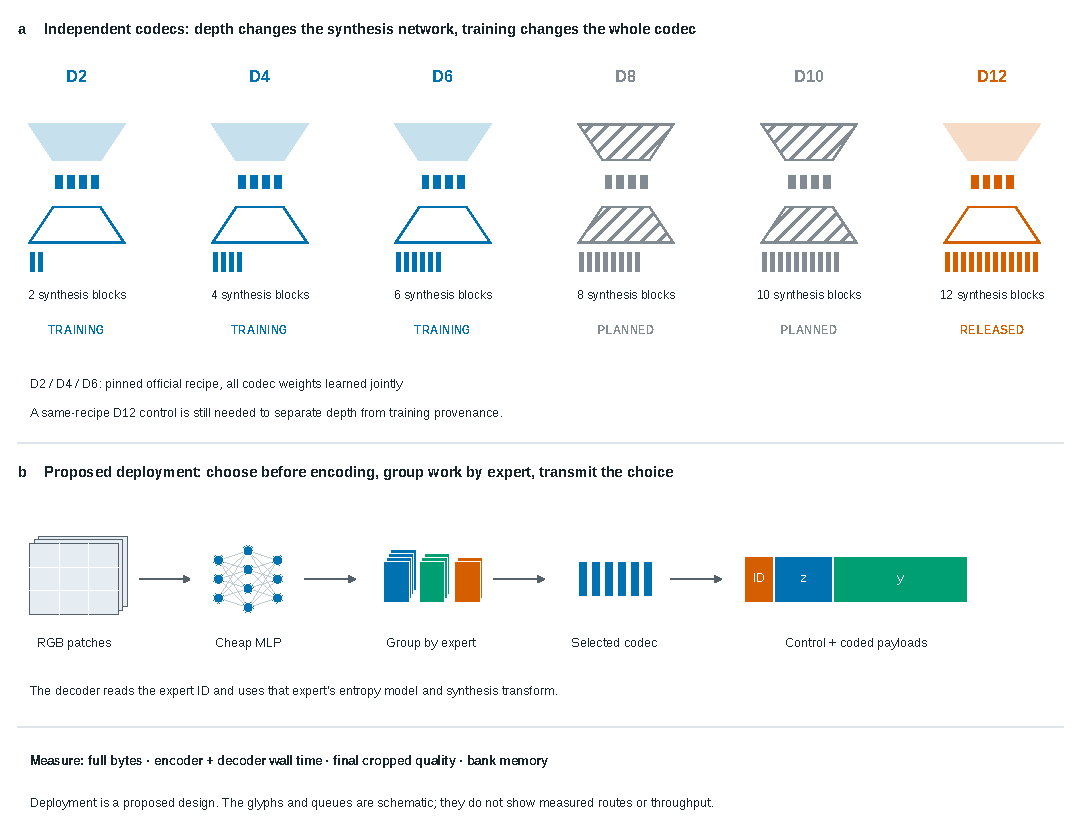
\includegraphics[width=\textwidth]{figs/extended20260927/figS3_codec_bank_plan.pdf}
\caption{\textbf{An independent codec bank is a separate experimental system.}
Training status is shown as of 27 September 2026. D2/D4/D6 are in progress,
D8/D10 are planned, and D12 is the released reference. Each expert owns its
analysis, entropy and synthesis parameters. The proposed encoder-side MLP
selects an expert before encoding; the decoder receives the expert ID.
Queues, network shapes and stream segments are schematic. No throughput or
quality result is encoded by their geometry.}
\label{fig:bank}
\end{figure*}

\section{Evaluation Contract for the Next Stage}

Expert training, router training, calibration and final evaluation should be
split at image level. Patches from the same image must stay in one split.
The four fixed validation crops in the current training monitor are health
checks; a broader intermediate evaluation should use the available 100
DIV2K validation images, followed by the declared final Kodak/CTC/CLIC
scope. This expanded evaluation is proposed and has not been completed.

Each codec needs a true-byte rate--distortion curve. Equal QP does not imply
equal rate across independently learned codecs. Comparisons should use their
common measured support, reporting infeasible targets and avoiding
extrapolation. Rate includes main and hyperprior payloads, model identity,
quality/control parameters and framing headers, divided by original pixels.
Quality is measured after cropping valid pixels; the exact RGB/YUV formula
and perceptual metrics are declared before test-set selection.

Timing requires the same GPU, precision, kernel path and warmup, with
alternated paired execution order and retained raw trials. Encoder,
decoder and complete round-trip times are separate outcomes. CUDA-event
module time and end-to-end wall time must remain separately labelled.
Grouping, scatter/gather, entropy work, stream parsing, transfers and fallback
are included where they occur. The full codec bank's resident weight memory
and peak activation memory are both reported.

The primary success criterion is a positive net runtime advantage over the
best validation-selected blind control on common achieved rate--distortion
support. Critical comparisons should then be repeated across training
seeds. A content bootstrap at fixed weights measures a different source of
variation and cannot replace those repeats.

\clearpage
{\small\bibliographystyle{ieeenat_fullname}\bibliography{main}}
\end{document}
